\section{CTF estimation}
 \begin{figure}[H]
  \centering
  \captionsetup{width=.8\linewidth} 
  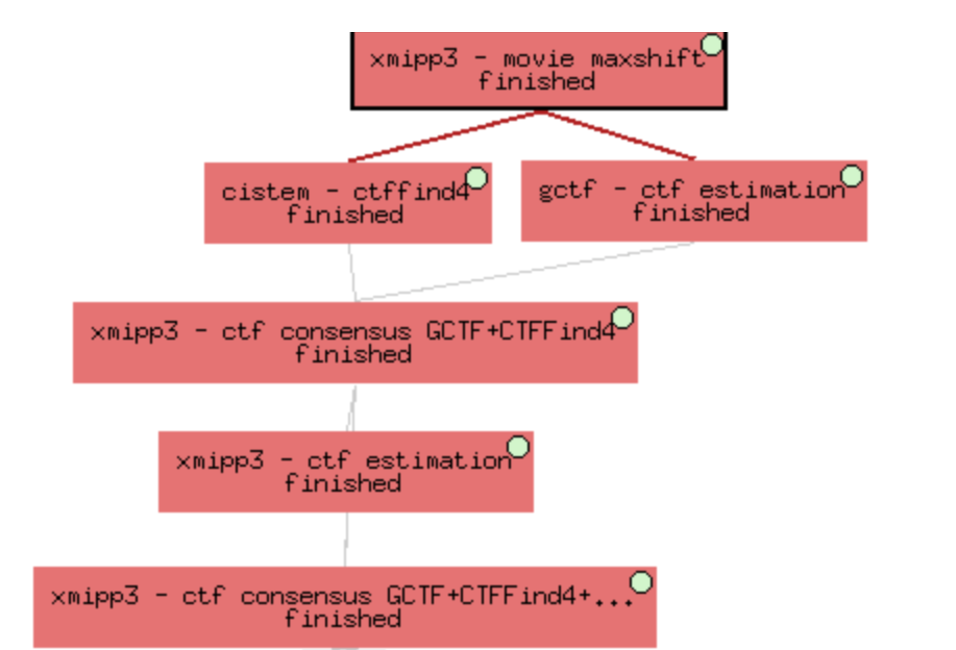
\includegraphics[width=0.45\textwidth]
  {{images/4_workflow2_CTFestimation.pdf}}
  \caption{CTF estimation workflow.}
  \label{fig:workflow_2}
  \end{figure}
  
Since close to focus images of biological specimens embedded in vitreous ice generate very little contrast, we take our movie-frames out of focus, and retrieve systematically distorted images of our specimens. The alteration observed is due to the different transference of contrast for each frequency. In an ideal microscope all the frequencies are transferred with total contrast (+1). In a normal one, some frequencies are transferred with contrast 0 or even -1. The CTF (Contrast transfer function) indicates how much contrast is transferred to the image as a function of the spatial frequency. The estimation of the CTF is the first step to correct it, repair its negative effect and retrieve our specimens undistorted.\\

How to estimate the CTF?\\

Since part of the Fourier components are lost, attenuated or inverted, images of the specimens taken in a non-ideal microscope will appear blurry. We define this blurry effect with the PSF (Point spread function). The effect of the PSF makes that a discrete point in the specimen is reproduced in the image as a broad point with a complex shape. The PSF can be directly estimated from the micrographs and, since the PSF and the CTF are related through the Fourier Transform, by computing the Fourier Transform of the PSF, we can directly estimate the CTF.\\

We count on different protocols to estimate the CTF of the micrographs in \scipion. In this tutorial we are going to use three different algorithms: \ttt{Gctf}\citep{gctf2016}, \ttt{CTFFind4} \citep{ctffind42015} and \ttt{Xmipp CTF estimation} \citep{sorzano2013semiautomatic} executed with protocols \scommand{gctf-ctf estimation} (\ffigure{fig:gctf_ctf_estimation}), \scommand{cistem-ctffind4}(\ffigure{fig:cistem-ctffind4}) and \scommand{xmipp3-ctf estimation}(\ffigure{fig:xmipp3_ctf_estimation}), respectively. Besides of estimating the CTF envelope, this last protocol improves the CTF estimation of \ttt{CTFFind4}. Thus, in this case an additional parameter is the defoci from a \ttt{Previous CTF estimation}. \\

\begin{figure}[H]
  \centering
  \captionsetup{width=.8\linewidth} 
  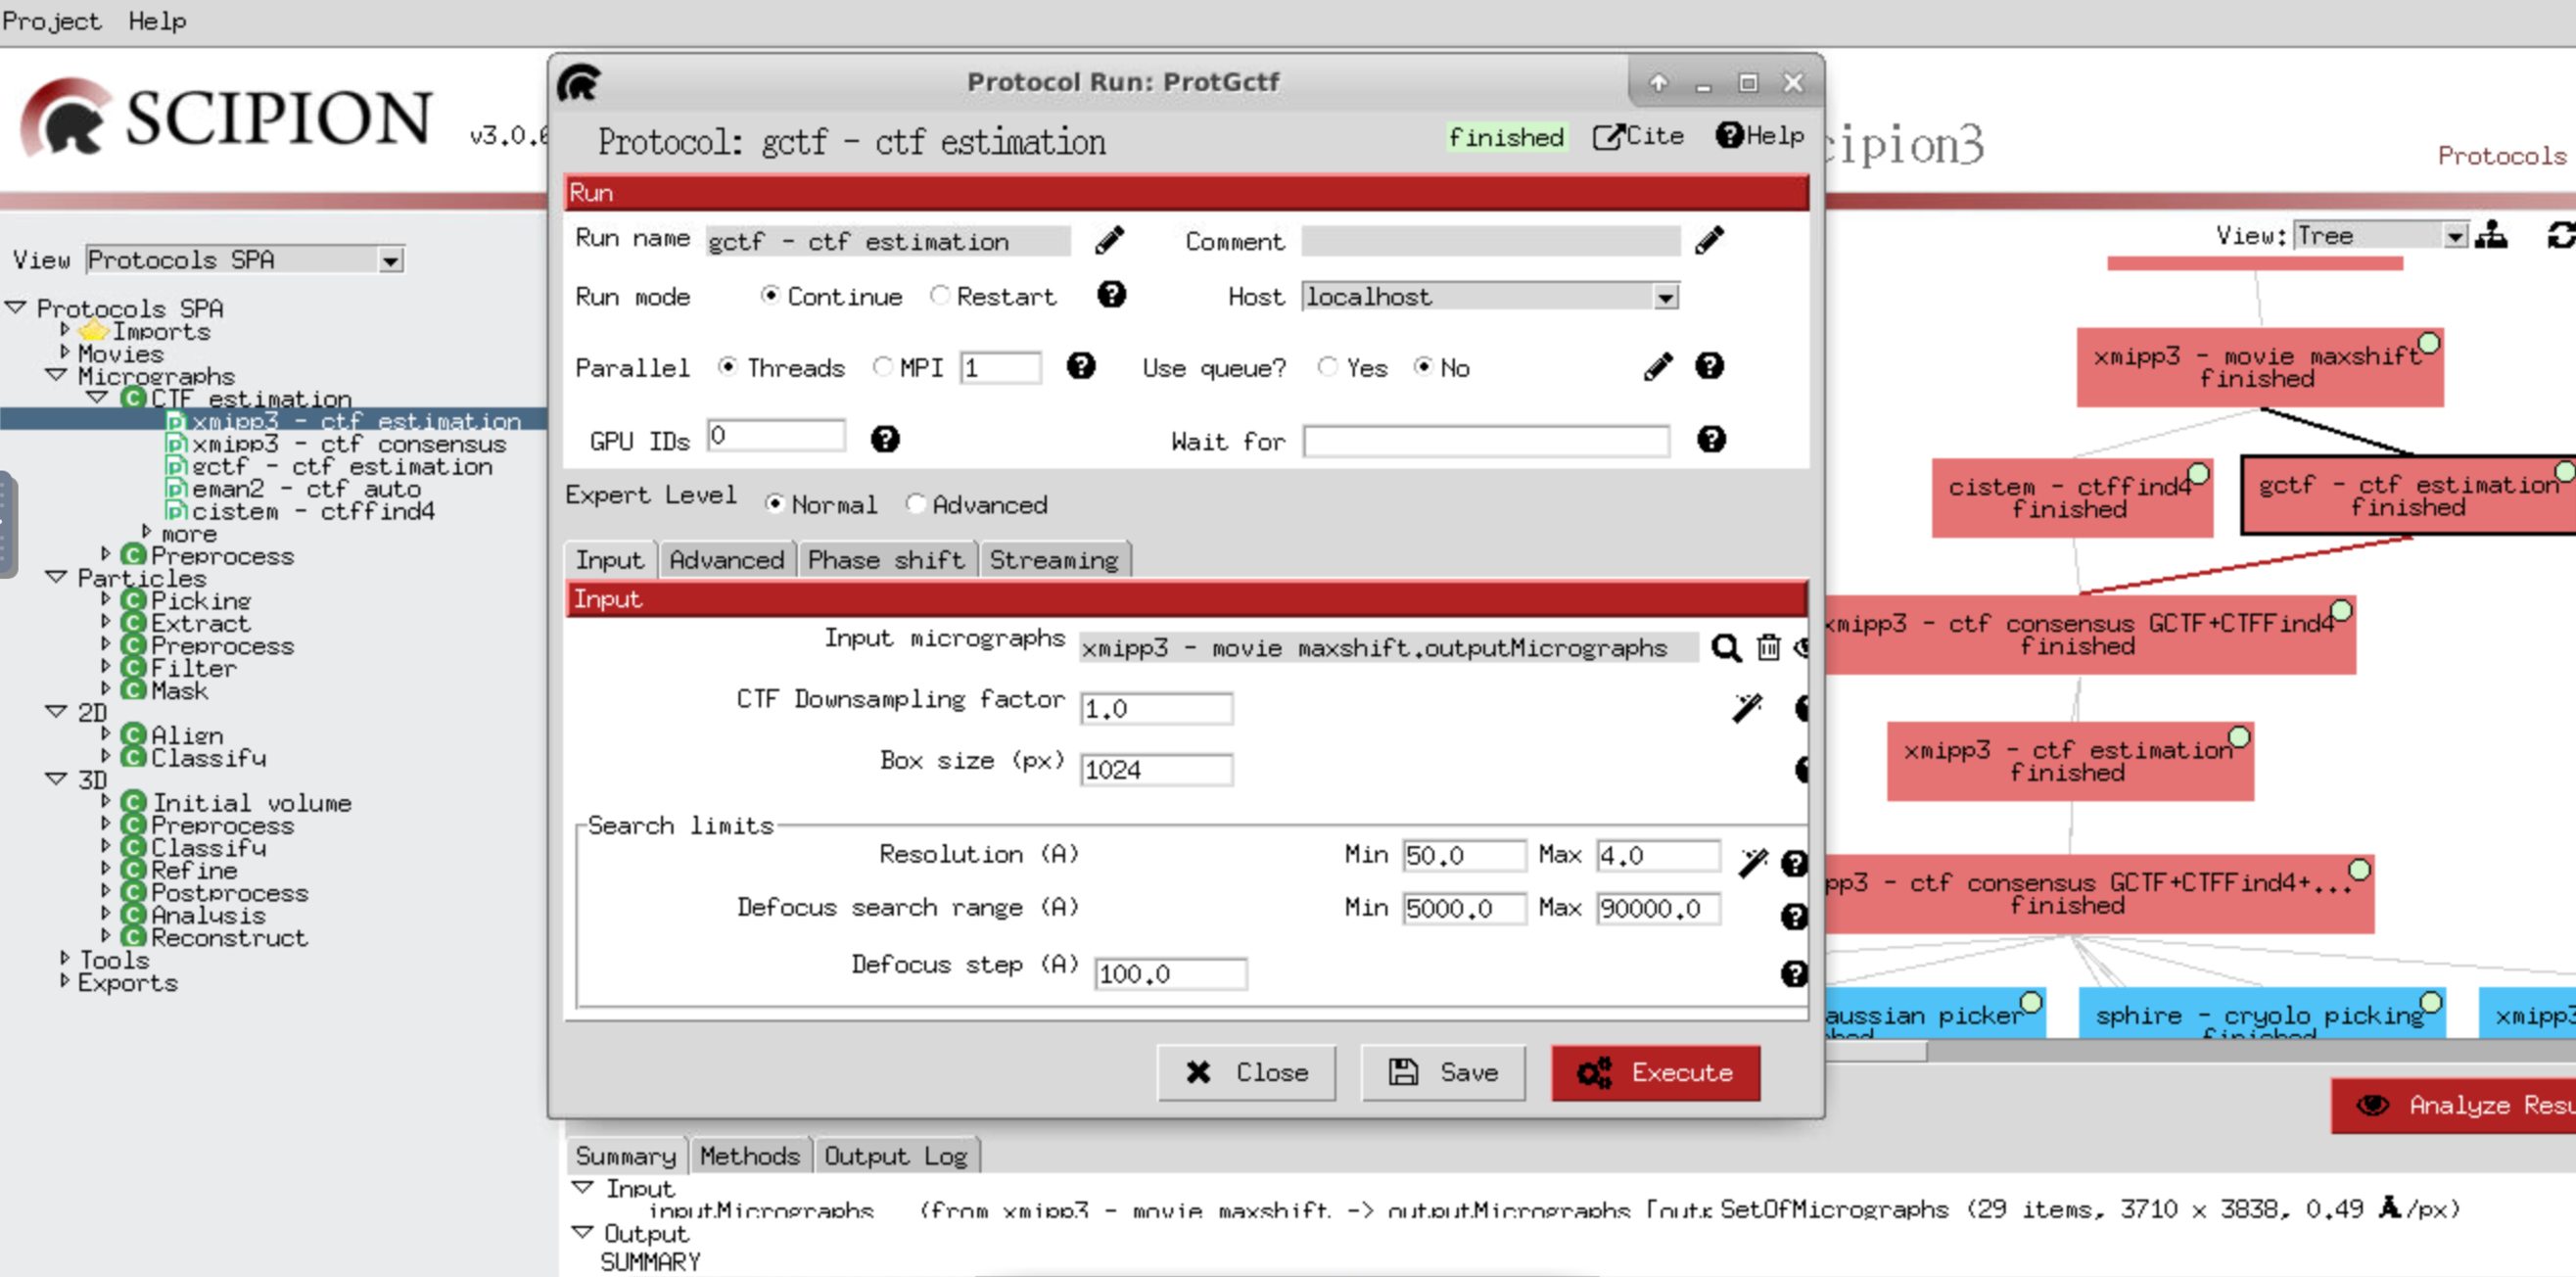
\includegraphics[width=0.95\textwidth]
  {{images/4b_gctf_ctfestimation.pdf}}
  \caption{Protocol 1 \scommand{gctf-ctf estimation} to compute the CTF.}
  \label{fig:gctf_ctf_estimation}
  \end{figure}
  
  \begin{figure}[H]
  \centering
  \captionsetup{width=.8\linewidth} 
  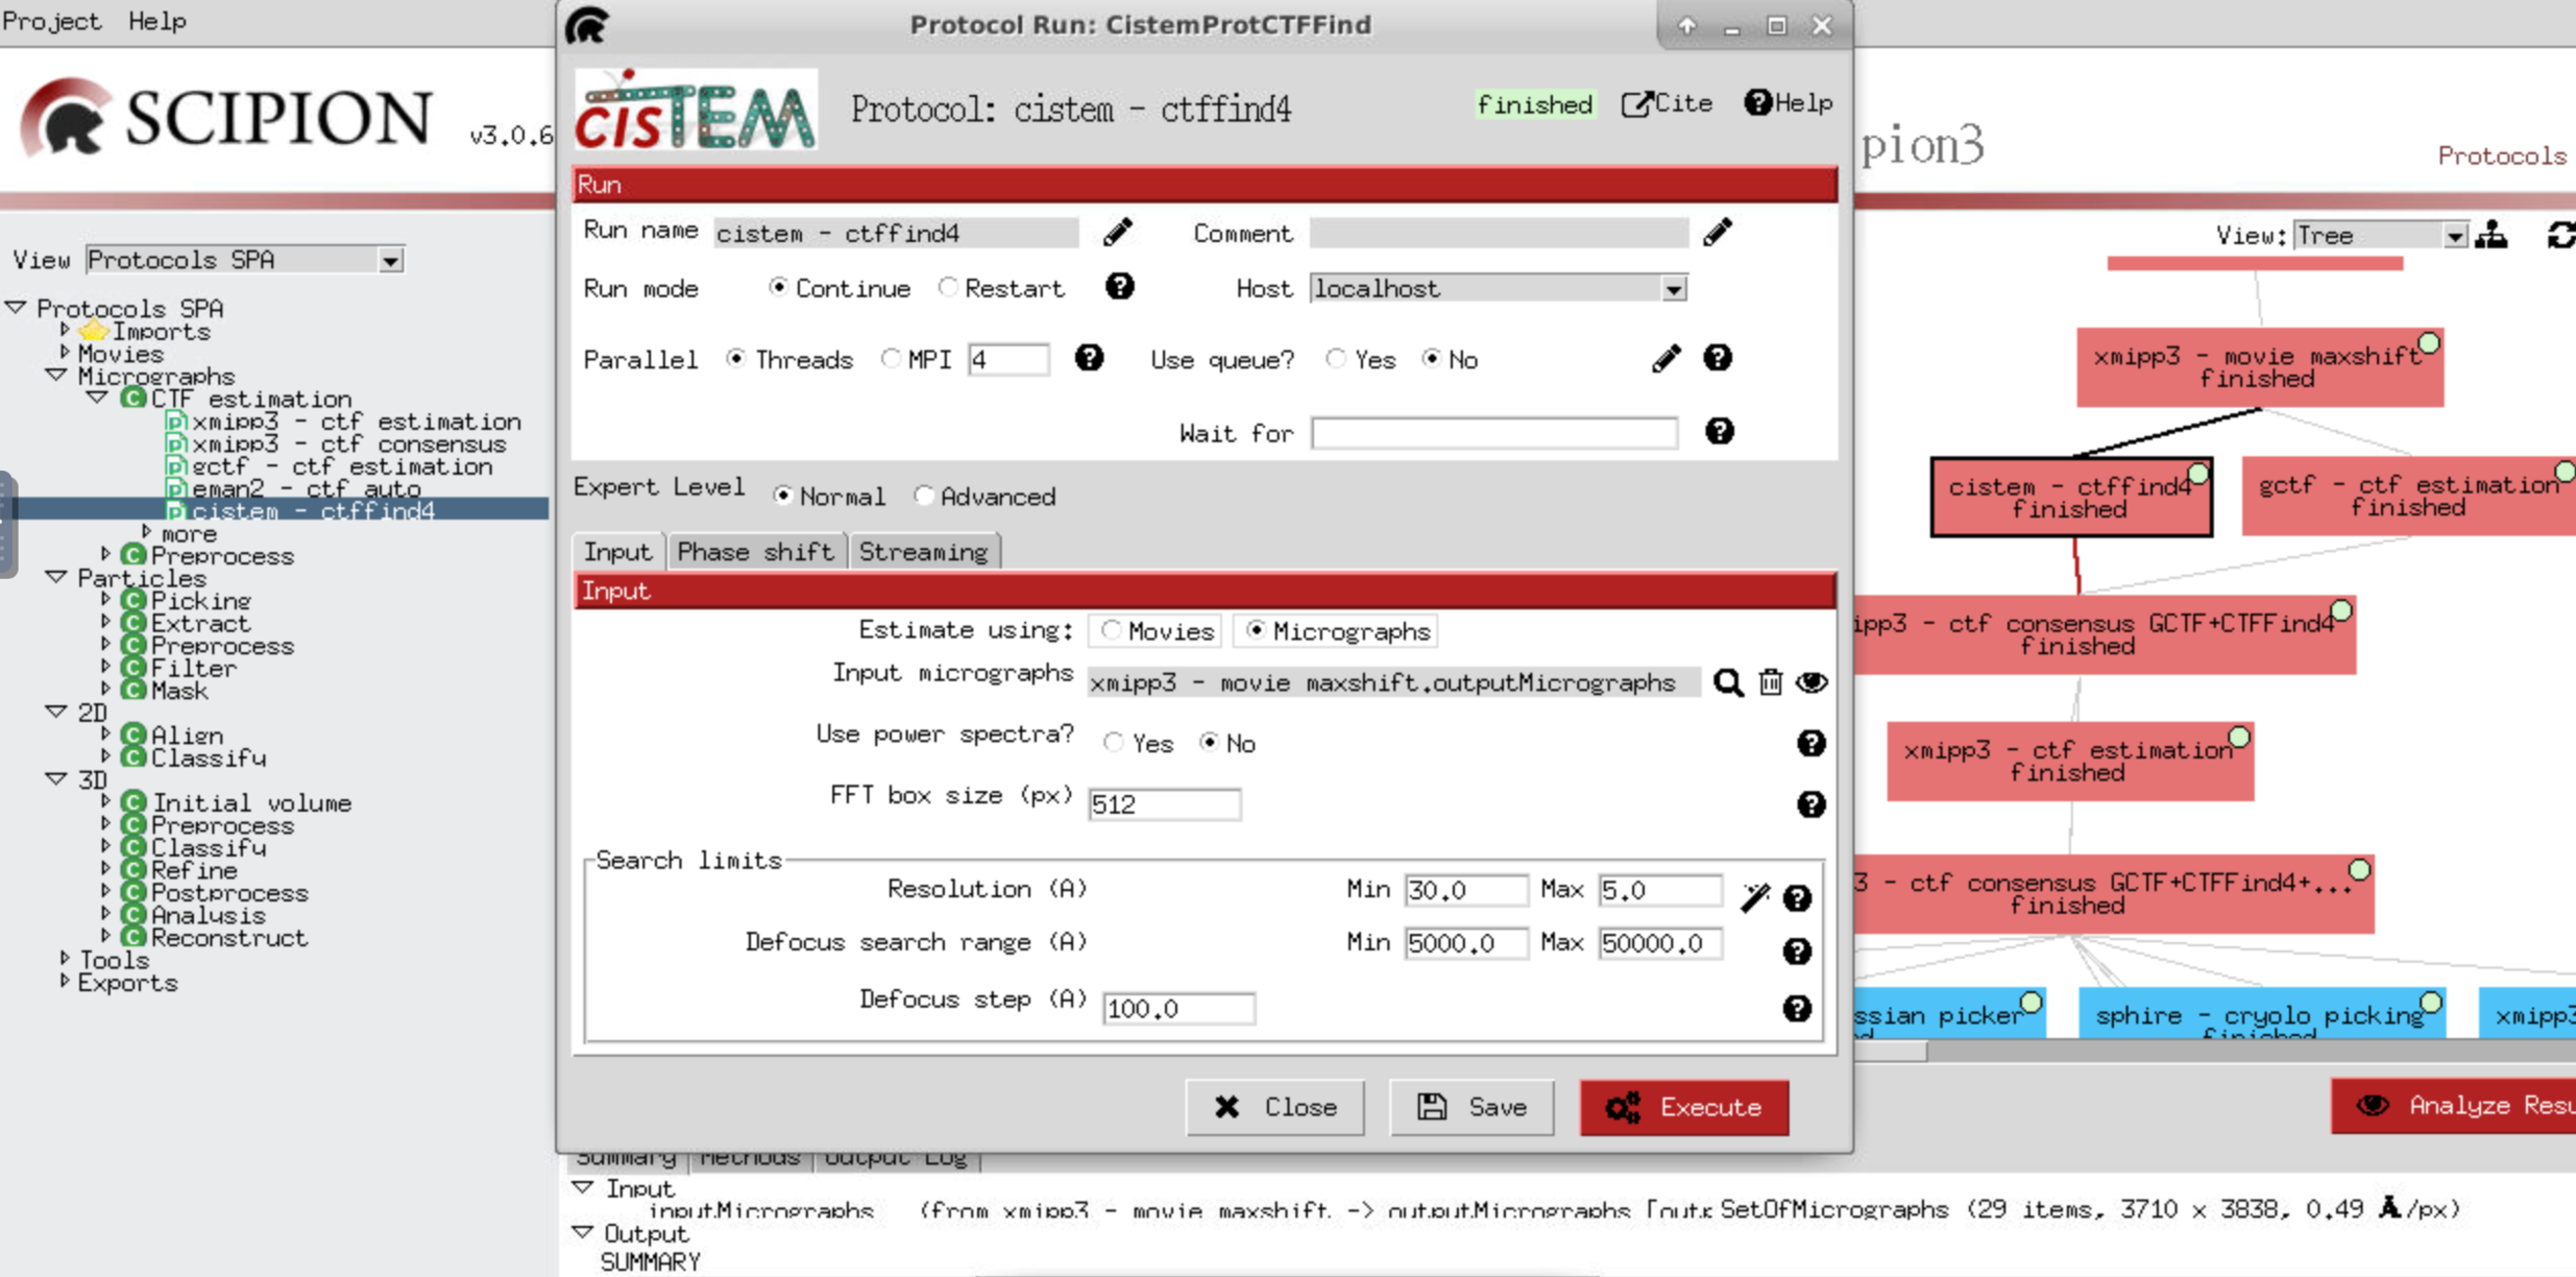
\includegraphics[width=0.95\textwidth]
  {{images/4a_cistem_ctffind4.pdf}}
  \caption{Protocol 2 \scommand{cistem-ctffind4} to compute the CTF.}
  \label{fig:cistem-ctffind4}
  \end{figure}
  
  \begin{figure}[H]
  \centering
  \captionsetup{width=.8\linewidth} 
  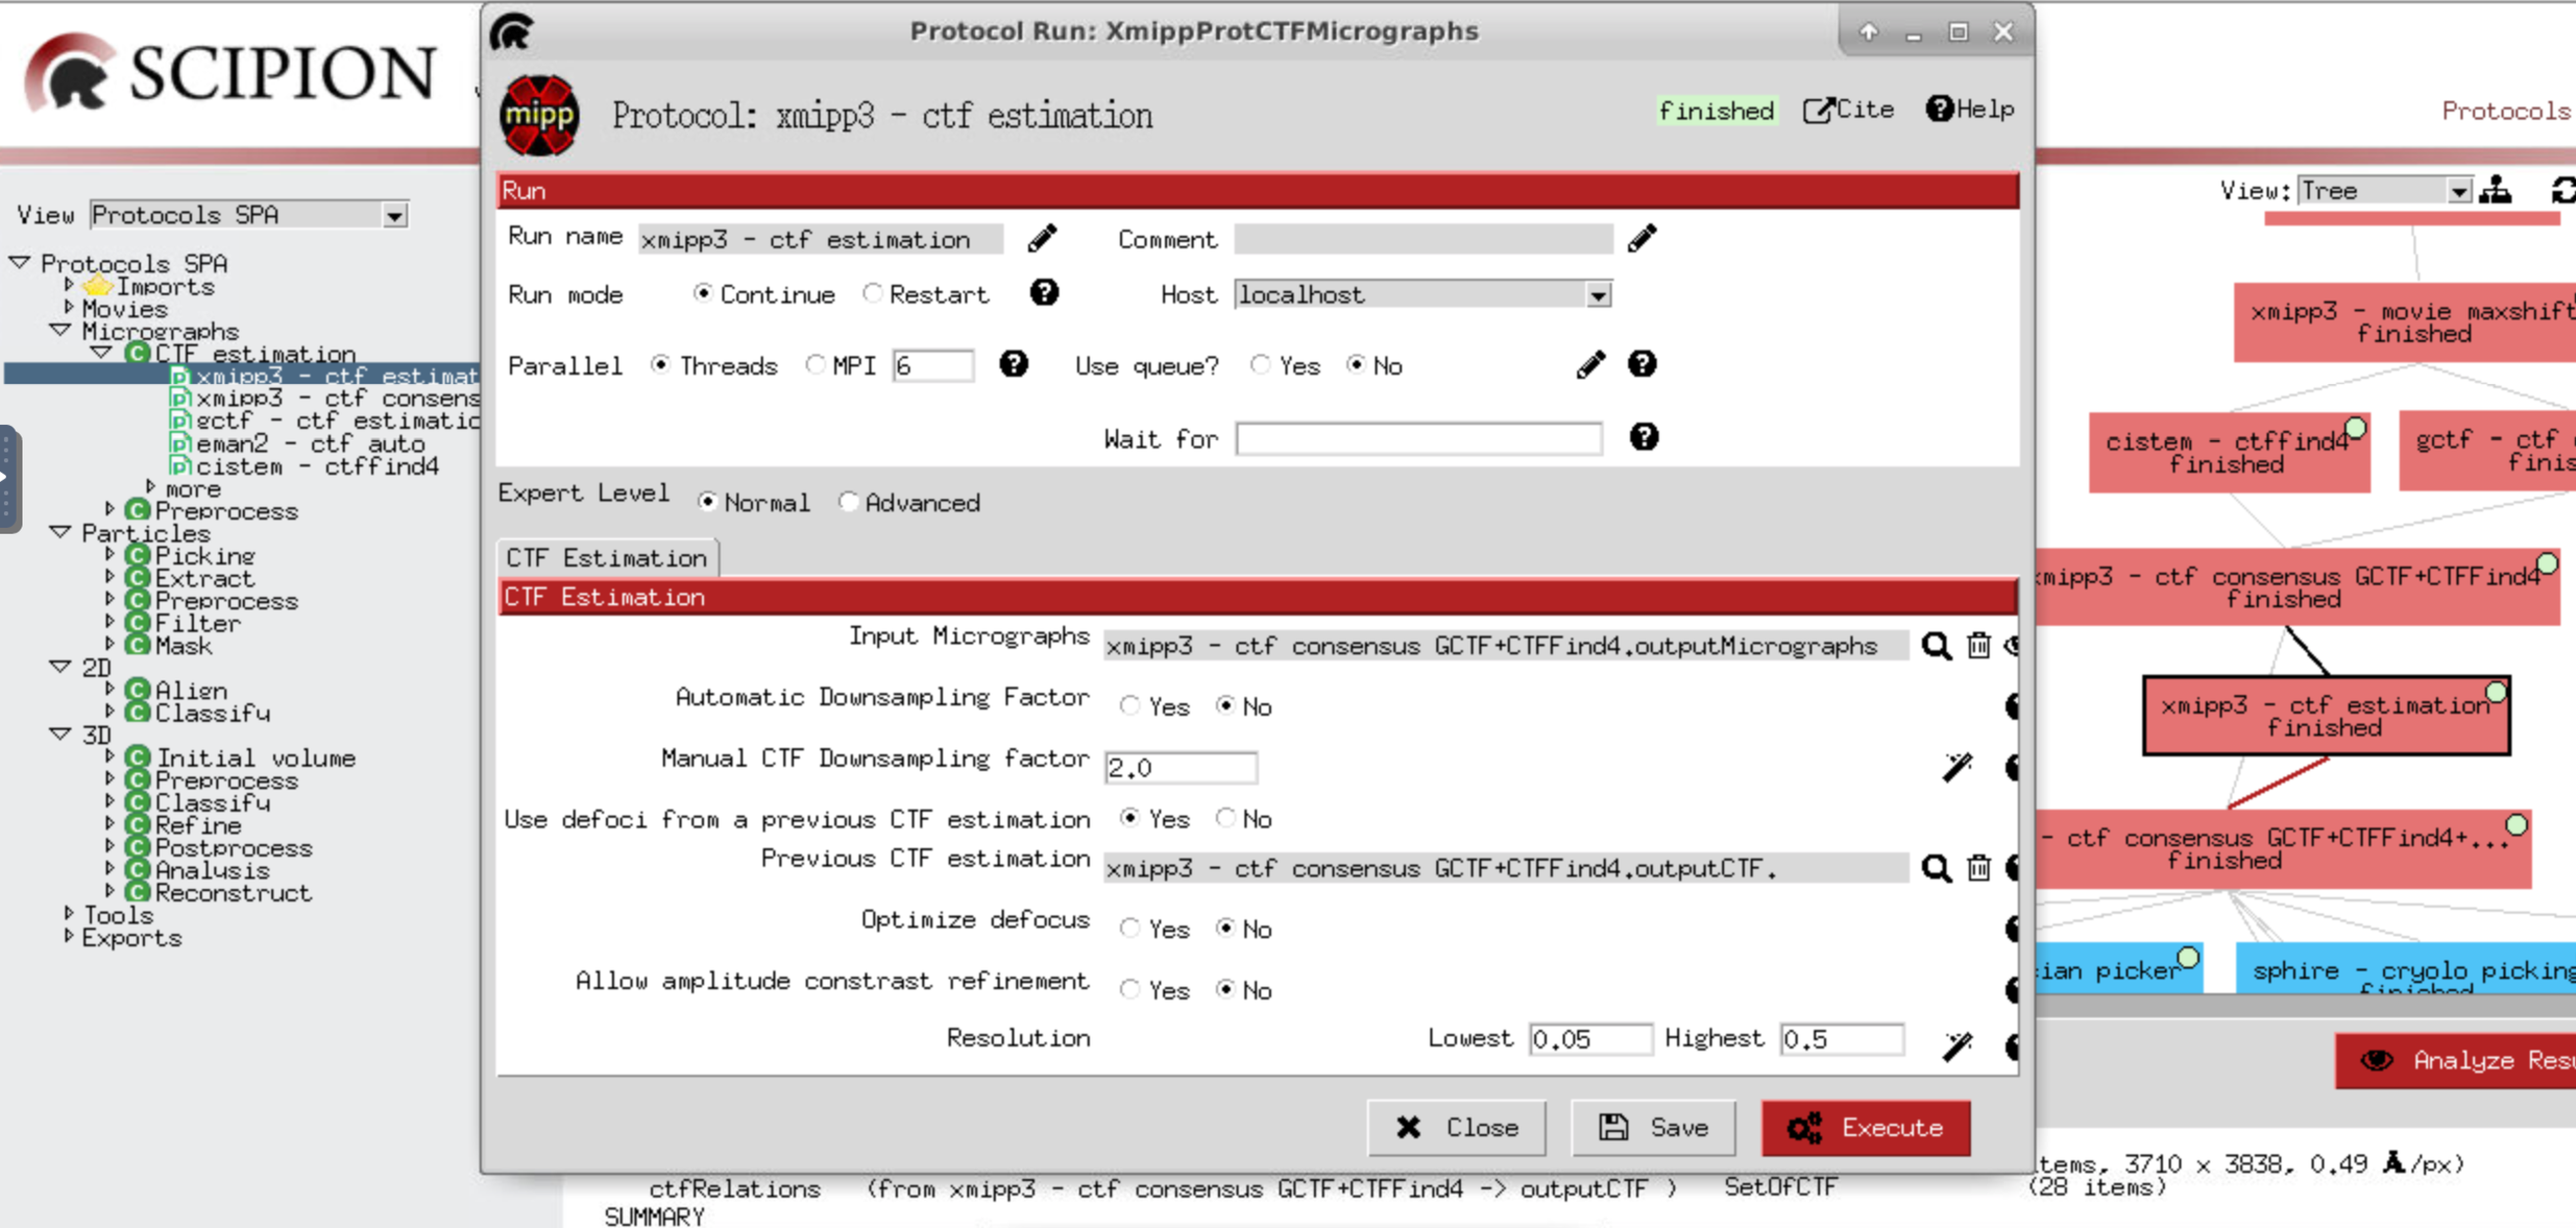
\includegraphics[width=0.95\textwidth]
  {{images/4d_xmipp3_ctfestimation.pdf}}
  \caption{Protocol 3 \scommand{xmipp3-ctf estimation} to compute the CTF.}
  \label{fig:xmipp3_ctf_estimation}
  \end{figure}
  
The three algorithms estimate the PSD of the micrographs and the parameters of the CTF (defocus U, defocus V, defocus angle, etc.). They cut micrographs into many smaller images with a desired window size. After that, they compute the Fourier Transform of each image and calculate an average. The three protocols designed to apply the three respective algorithms contain very similar parameters. To estimate the CTF we need to limit the frequency region to be analyzed between the lowest and highest resolution. The frequency domain selected must include all zeros of the CTF. The wizard displayed on the right helps to choose that frequency region.\\

After executing each one of these three protocols, results can be observed by pressing \scommand{Analyze results}. A table will be opened showing the image of the CTF computed for each micrograph, as well as other CTF parameters. CTFs of good micrographs typically display multiple concentric rings extending from the image center towards its edges. Bad micrographs, however, might lack rings or show very few of them that hardly extend from the image center. Micrographs like these will be discarded, likewise micrographs showing strongly asymmetric rings (astigmatic) or rings that attenuate in a particular direction (drifted). To discard a particular micrograph, select it, clik the mouse right button and choose \ttt{Disable}. If you want to see the CTF profile, choose the option \ttt{Show CTF profile}, and a new window will be opened to show the CTF profile. \ttt{Recalculate CTFs} and \ttt{Micrographs} are additional options of \scommand{Analyze results} menu that can be used after selecting specific micrographs. \ttt{Recalculate CTFs} allows to estimate again the CTF when the algorithm has previously failed to find the rings, even if they can be seen by eye. The option \ttt{Micrographs} allows to create a new subset of selected micrographs.\\

Concerning some differences among protocols, we remark that micrographs with CTF estimated with \scommand{cistem-ctffind4} display a hole in the center because, in some cases, they have very much power and avoid appreciate what is underneath. In the particular case of \scommand{xmipp3-ctf estimation}, four different images of micrographs are shown. Besides the PSD, this last protocol displays the enhanced PSD, the CTF model by quadrants and half planes.\\

\subsection*{CTF consensus}
The CTF estimation process concludes by applying two different consensus protocols to assess first, the differences among the output of the algorithms \ttt{Gctf} and \ttt{CTFFind4} and second, the differences among the consensus reached by those two and \ttt{Xmipp CTF estimation}. We are going to use \scommand{xmipp3-ctf consensus} to perform this task (\ffigure{fig:xmipp3-ctf_consensus_1} and \ffigure{fig:xmipp3-ctf_consensus_2}). This protocol allows to screen micrographs according meaningful CTF estimations based on defocus values, astigmatism, resolution and other \ttt{Xmipp} criteria (second tap in the protocol form), which will only be used in case that any of the CTFs computed is estimated by \scommand{xmipp3-ctf estimation}.\\

\begin{figure}[H]
  \centering
  \captionsetup{width=.8\linewidth} 
  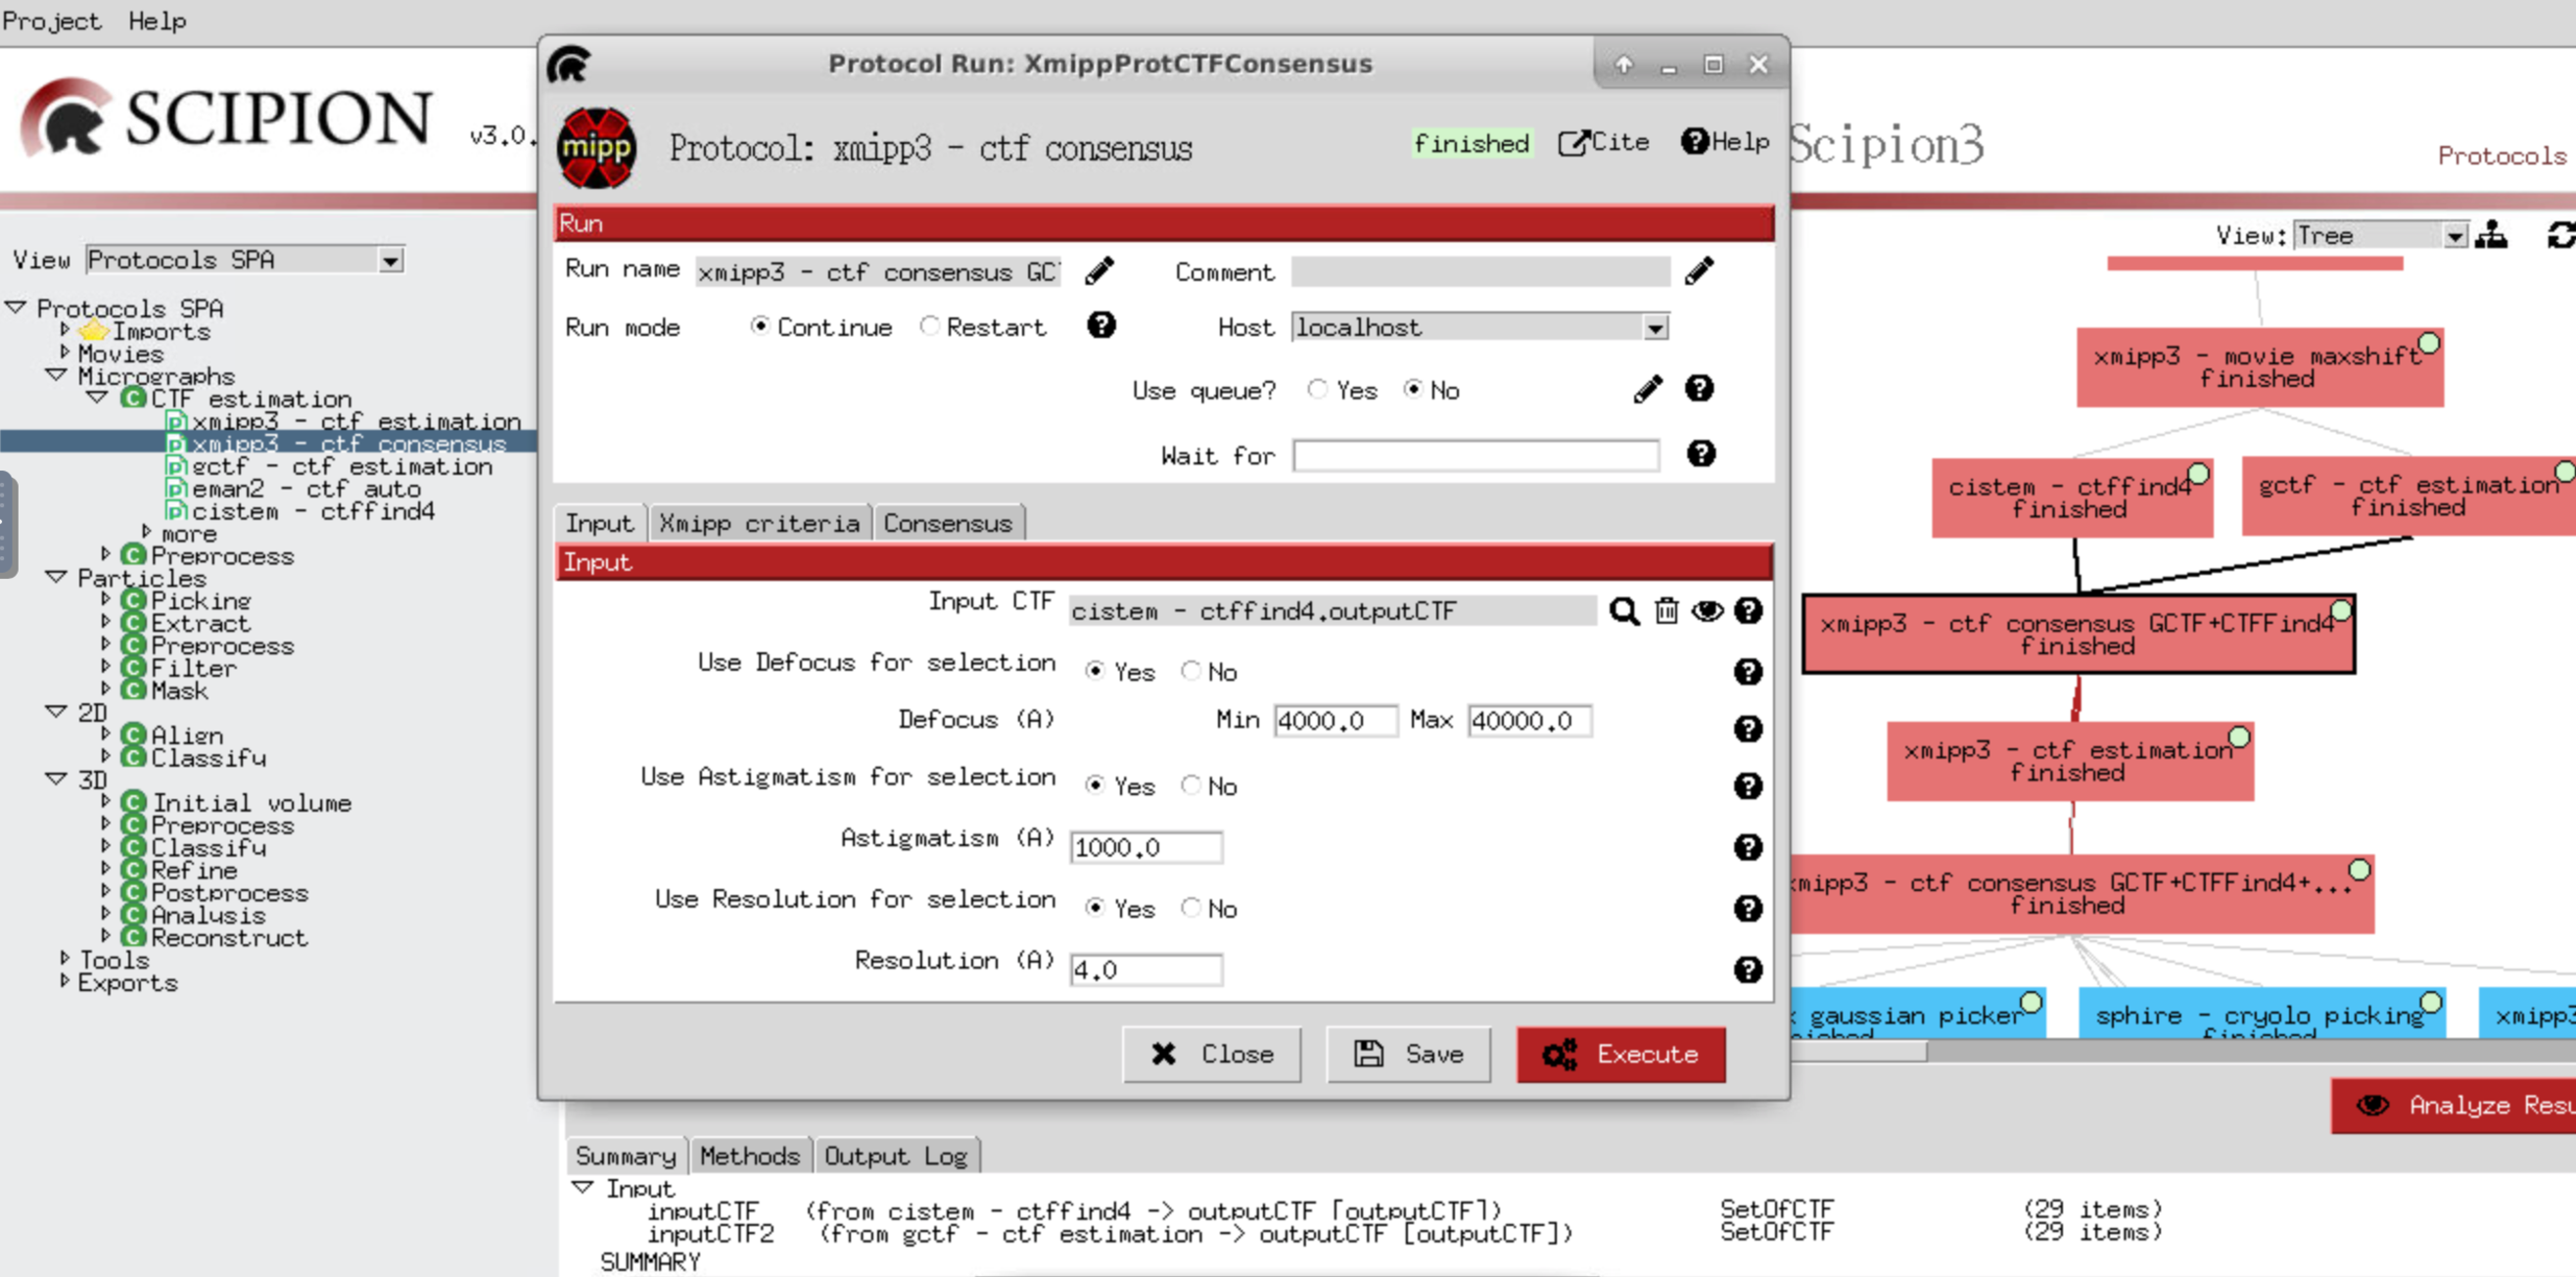
\includegraphics[width=0.95\textwidth]
  {{images/4c_xmipp3_ctfconsensus.pdf}}
  \caption{Filling in the consensus protocol 1 \scommand{xmipp3-ctf consensus}.}
  \label{fig:xmipp3-ctf_consensus_1}
  \end{figure}

In this first case we have selected, as first input, the estimation of the CTF calculated by \scommand{cistem-ctffind4} and, as second input, the estimation obtained by \scommand{gctf-ctf estimation}. By pressing \scommand{Analyze Results} both accepted (28) and rejected (1) micrographs can be visualized. This consensus was used to obtain a good estimate of the defocus.\\

\begin{figure}[H]
  \centering
  \captionsetup{width=.8\linewidth} 
  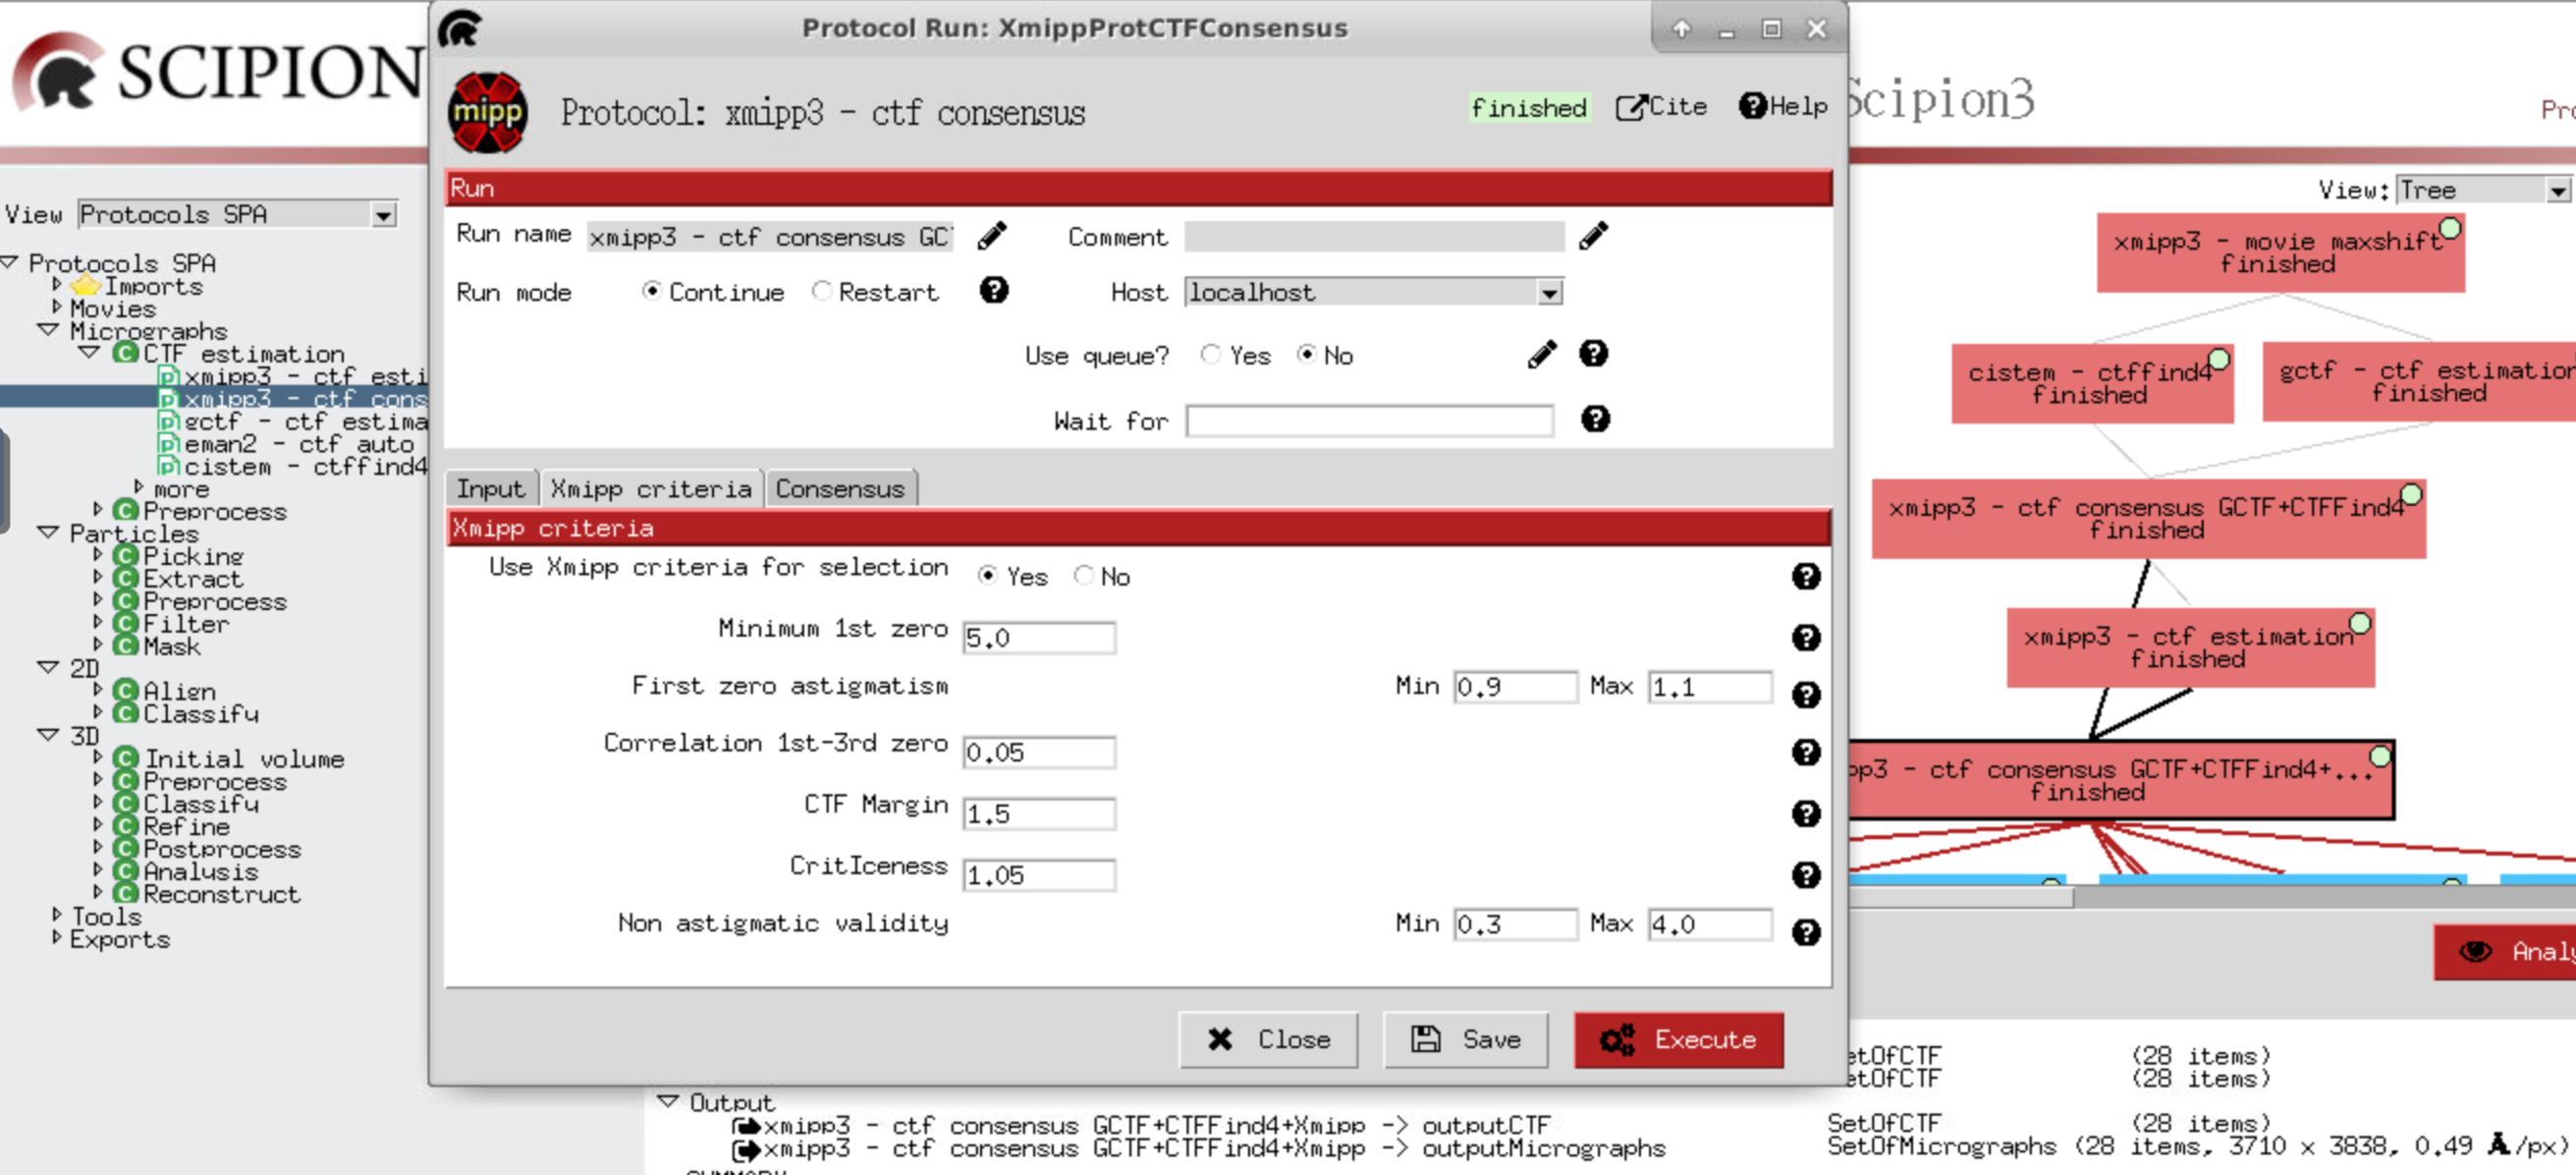
\includegraphics[width=0.95\textwidth]
  {{images/4e_xmipp3_ctfconsensus2.pdf}}
  \caption{Filling in the consensus protocol  2 \scommand{xmipp3-ctf consensus}.}
  \label{fig:xmipp3-ctf_consensus_2}
  \end{figure}
  
 In this second case we have selected, as first input, the estimation of the CTF calculated by \scommand{xmipp3-ctf estimation} and, as second input, the estimation obtained by \scommand{xmipp3-ctf consensus GCTF and CTFFind4}. By pressing \scommand{Analyze Results} both accepted (28) and rejected (0) micrographs can be visualized. On the other hand, once we had a good estimate of the defocus with this consensus we obtained a good estimate of the envelope.\\ 

With the proper set of micrographs we can continue the image processing. The negative effects of the CTF will be corrected in the next steps.\\

For more information: 
\begin{itemize}
   \item \textbf{Video tutorial}: second half of this video \url{https://www.youtube.com/watch?v=O1sBrJbKh7I&list=PLQjWIcrmtc4JjyC-_BM99_XW-VsDa4_i3&index=26}.
   \item \textbf{Theoretical lecture}: second half of this video \url{https://www.youtube.com/watch?v=F3Uslh3v9J8&list=PLQjWIcrmtc4JjyC-_BM99_XW-VsDa4_i3&index=32}.
  \end{itemize}

